\begin{document}
Pel que fa a l'anàlisis de costos, s'ha intentat segregar segons els diferents paràmetres on el sistema es pot derivar, que són:
\begin{itemize}
	\item La mida del sistema agregat, és a dir, el nombre de comptadors d'un barri.
	\item L'algorisme emprat per tal de realitzar el logaritme discret.
\end{itemize}
No obstant això, anteriorment s'ha especificat certes propietats que comporta el sistema:
\begin{itemize}
	\item Es considera que entre ronda i ronda hi haurà, com a mínim, un interval de 15 minuts, és a dir, la lectura que es passarà correspondrà al consum dels últims 15 minuts.
	\item Per tal de no sobrecarregar l'algoritme del logaritme discret, les lectures dels comptadors han de tenir un cert grau de control en la seva mida en bits.\\
	 Primer, es va pensar realitzar l'anàlisis amb lectures pseudo-aleatòries. Per aquesta raó, està creada la classe \texttt{RandomConsumption}, que enviava un enter positiu aleatori de, com a màxim, 13 bits. Aquesta classe ens servirà per poder comparar els diferents protocols o realitzar funcions estadístiques, ja que les lectures no es comportaran diferent segons la ronda quan s'envien.\\
	 No obstant això, amb la intenció de tenir una simulació més realista, s'ha buscat un \textit{dataset} que ens permeti visualitzar el consum elèctric d'una llar \cite{kaggle-consumption} i crear un lectures més properes a les reals. Aquestes dades ens serviran per poder veure fins quan el cost de realitzar el logaritme discret és factible.\\
	 Les dades trobades aporten el consum elèctric amb una freqüència de mostreig d'un minut durant aproximadament 4 anys en tres espais diferents de la llar, tal i com es pot apreciar a la \textit{Taula \ref{tab:ex-kaggle}}.
	\begin{table}[H]
		\centering
			\begin{tabular}{llrrr}
				\toprule
				{} &           date\_time &  Sub\_metering\_1 &  Sub\_metering\_2 &  Sub\_metering\_3 \\
				\midrule
				0 & 2006-12-16 17:24:00 &             0.0 &             1.0 &            17.0 \\
				1 & 2006-12-16 17:25:00 &             0.0 &             1.0 &            16.0 \\
				2 & 2006-12-16 17:26:00 &             0.0 &             2.0 &            17.0 \\
				3 & 2006-12-16 17:27:00 &             0.0 &             1.0 &            17.0 \\
				4 & 2006-12-16 17:28:00 &             0.0 &             1.0 &            17.0 \\
				...\\
				\bottomrule
			\end{tabular}
		\caption{Primeres files del dataset.}
		\label{tab:ex-kaggle}
	\end{table}
	Primer, s'han tractat les dades agregant els consums dels diferents espais per trobar el consum total de la llar. Seguidament, un cop tenint el consum de la llar agregat, es realitza la mitjana d'aquest valor en funció del temps, és a dir, la mitjana de tots els dies en funció de l'hora i el minut en què s'ha realitzat la lectura. Una part del resultat obtingut es mostra a la \textit{Taula \ref{tab:ex-kaggle-mean}}, com a exemple.
	\begin{table}[H]
		\centering
		\begin{tabular}{lrrr}
			\toprule
			{} & hour & min & consumption mean \\
			\midrule
			0 &    0 &   0 &    4.537868 \\
			1 &    0 &   1 &    4.524544 \\
			2 &    0 &   2 &    4.568022 \\
			3 &    0 &   3 &    4.599579 \\
			4 &    0 &   4 &    4.600281 \\
			5 &    0 &   5 &    4.666199 \\
			6 &    0 &   6 &    4.443198 \\
			7 &    0 &   7 &    4.525947 \\
			8 &    0 &   8 &    4.596073 \\
			...\\
			\bottomrule
		\end{tabular}
	\caption{Primeres files del dataset transformat realitzant la mitjana}
	\label{tab:ex-kaggle-mean}
	\end{table}
	   Així doncs, es pot visualitzar la mitjana trobada pel consum elèctric total de la llar en funció del horari de la següent forma:
\begin{figure}[H]
	\centering
	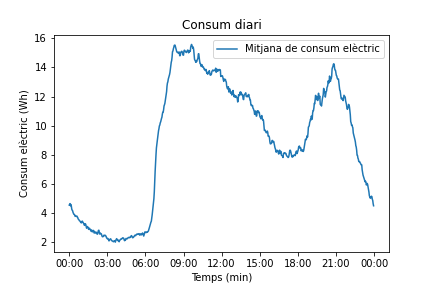
\includegraphics[width=8cm]{imgs/cost/consumptionmin.png}
	\caption{Mitjana de consum diari.}
	\label{fig:consumptionmin1}
\end{figure}
Per tal de variar les lectures entre diferents comptadors, s'ha creat una cota màxima i una cota mínima per establir un rang de possibilitats:
\begin{figure}[H]
	\centering
	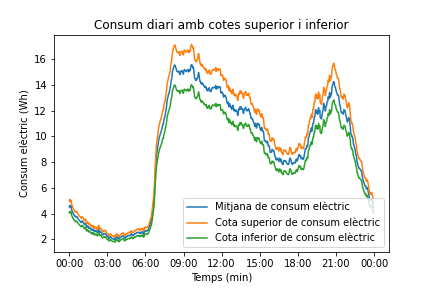
\includegraphics[width=8cm]{imgs/cost/consumptionmin2.png}
	\caption{Mitjana de consum diari amb cotes superior i inferior.}
	\label{fig:consumptionmin2}
\end{figure}
Finalment,  s'han agregat els consums de 15 en 15, ja que la lectura es passarà en intervals de 15 minuts, com ja s'ha mencionat anteriorment. D'aquesta manera, cada quart d'hora correspon a una classe d'equivalència. \\
En conclusió, es pot afirmar que agafant un nombre pseudo-aleatori dins del rang possible corresponent a cada ronda, es pot acabar generant un dia de lectures més o menys fidel a la realitat. No obstant això, cal esmentar que s'ha modificat lleugerament la cota superior per tal de crear més variació entre comptadors, tal i com es pot veure a la \textit{Figura \ref{fig:consumption2}}.
\begin{figure}[H]
	\centering
	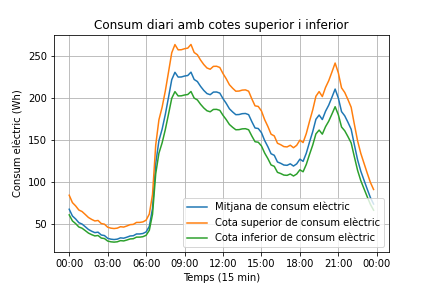
\includegraphics[width=8cm]{imgs/cost/consumption2.png}
	\caption{Gràfica de lectures amb cotes superior i inferior.}
	\label{fig:consumption2}
\end{figure}
Com es pot observar, les lectures mai seran d'una mida superior a $13$ bits, ja que $log_2(v_{max}) = log_2(263) = 8.04$. Sabent això, el missatge xifrat agregat serà d'una llargada màxima de $|D_2|_{max} = 8 + \lceil log_2(N) \rceil$ sent $N$ el nombre de comptadors intel·ligents al barri.
\end{itemize}
Es pot veure el tractament del \textit{dataset} i de les dades obtingudes en l'anàlisis de cost en el repositori remot \cite{lab-recsi}.
\section{Algorismes de computació del logaritme discret}
El primer que es voldrà analitzar seran els diferents algoritmes implementats que realitzen el logaritme discret, que són un total de tres:
\begin{itemize}
	\item Pollard's Lambda, descrit a la \textit{Secció \ref{sec:pollards}}.
	\item Algoritme de força bruta \texttt{BruteForce}, on el generador passa pels possibles elements del grup fins trobar la potència. Aquest algoritme es va utilitzar per realitzar diversos tests i s'ha cregut encertat comparar-lo amb el Pollard's Lambda.
	\item Algoritme \textit{singleton} de força bruta \texttt{HashedAlgorithm}, on es realitza un cop l'algoritme per guardar les relacions entre tots els elements i la seva respectiva potència. De manera que, si es carrega la classe abans, l'únic cost a l'hora de realitzar el logaritme discret serà l'accés a memòria. No obstant el cost del temps és més reduït, la memòria que ocupa és bastant gran i es necessita un temps inicial per construir la taula. Al final, el que tindrem a l'hora de cridar el mètode serà un \textit{HashMap} que, donat un element $a \in \mathbb{Z}_p$ o  $A \in E(\mathbb{Z}_p)$ ens retornarà la seva clau $k$, sabent que:
	\[g^k = a ,\quad \textrm{ usant  }\ \mathbb{Z}_p\]
	\[G \cdot k = A,\quad \textrm{ usant  }\ E(\mathbb{Z}_p)\]
\end{itemize}
L'anàlisis del protocol en funció dels algoritmes s'ha dut a terme usant un processador \texttt{AMD A6-6310 APU @ 1800GHz} de $4$ nuclis. El generador de lectures usat és el \texttt{RandomConsumption} per tenir la mateixa configuració pel que fa a la llargada dels missatges, ja sigui en \textit{KT} com \textit{CT}. A l'hora d'analitzar en funció de l'algoritme \texttt{BruteForce}, a causa del temps que requereix per realitzar el logaritme discret, només s'ha repetit el cas 20 vegades. Per aquest motiu possiblement, veiem a la \textit{Taula \ref{tab:brute}} que el temps és major a \textit{CT }que \textit{KE}, ja que no hi ha suficients dades.
	\begin{table}[H]
		\centering
		\begin{tabular}{lrrrrr}
			\centering
			&\multicolumn{5}{l}{\centering Temps (ms)}\\
			\toprule
			Num meters: &           3  &       4  &           5  &            8  &            16 \\
			\midrule
			ct &  4057.700 &  5000.48 &  5810.060 &  11039.280 &  26033.700 \\
			ke &  3337.867 &  4277.60 &  5361.467 &  10282.867 &  20808.467 \\
			\bottomrule
		\end{tabular}
		\caption{Cost experimental del protocol usant \texttt{BruteForce}.}
		\label{tab:brute}
	\end{table}
Els resultats en \texttt{PollardsLambda} \ref{tab:pollards} i \texttt{HashedAlgorithm} \ref{tab:hashed} són molt més prometedors i verifiquen que el logaritme discret, en cas de no estar implementat de manera eficient, pot generar un coll d'ampolla.
\begin{table}[H]
	\centering
	\begin{tabular}{lrrrrrrrrr}
		\centering
		&\multicolumn{9}{l}{\centering Temps (ms)}\\
		\toprule
		Num meters: &           3  &       4  &           5  &            8  &              16  &         32  &         64  &      128 &     192 \\
		\midrule
		ct &  217.35 &  206.02 &  260.57 &  220.97 &  232.685 &  261.47 &  304.12&  407.07 &  485.48 \\
		ke &  249.53&  292.13&  305.13&  310.13&  297.06&  328.20 &  464.73&  680.86&  900.00 \\
		\bottomrule
	\end{tabular}
	\caption{Cost experimental del protocol usant \texttt{PollardsLambda}.}
	\label{tab:pollards}
\end{table}

	\begin{table}[H]
	\centering
	\begin{tabular}{lrrrrrrrrr}
		\centering
		&\multicolumn{9}{l}{\centering Temps (ms)}\\
		\toprule
		Num meters: &           3  &       4  &           5  &            8  &              16  &         32  &         64  &      128 &     192 \\
		\midrule
		ct &  18.83 &  19.57 &  22.93 &  28.10 &   43.77 &   70.63&  120.20 &  245.46 &  370.21 \\
		ke &  42.13&  60.20 &  56.26&  72.13&  114.40 &  175.26&  338.46&  563.20 &  758.80 \\
		\bottomrule
	\end{tabular}
	\caption{Cost experimental del protocol usant \texttt{HashedAlgorithm}.}
	\label{tab:hashed}
\end{table}
No obstant això, es pot observar que la funció de cost en tots els algoritmes és lineal i no exponencial, tal i com hauria de ser. Això és degut a les especificacions del processador, ja que només té 4 nuclis i no permet que els comptadors treballin de manera simultània. Això provoca que, al usar un nombre de processos més elevat que el de nuclis o \textit{threads virtuals}, en cas que en tingués, no es pot realitzar una simulació paral·lela. Gràcies a això també es pot explicar perquè la fase \textit{KE}, que és la que comporta més comunicació entre comptadors i subestació, és la fase més costosa usant els algoritmes \texttt{HashedAlgorithm} i \texttt{PollardsLambda}, on el cost del logaritme és més baix.
\\
\\
 A la \textit{Figura \ref{fig:comparisons}} es compara el cost del protocol en funció de \texttt{PollardsLambda} i \texttt{HashedAlgorithm}, no s'ha pogut comparar en aquest gràfic \texttt{BruteForce}, doncs el cost és molt més alt.
 Mentres que a la \textit{Figura \ref{fig:algorithms}} es pot veure el resultat de les taules de manera més gràfica.
\begin{figure}[H]
	\centering
	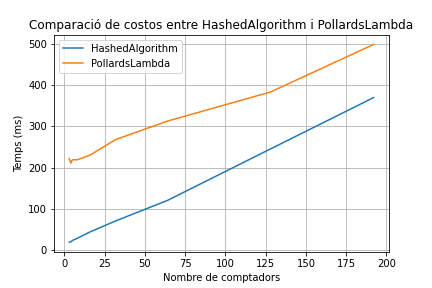
\includegraphics[width=7cm]{imgs/cost/comp-hashed-pollards.png}
	\caption{Comparació de rendiment del protocol entre els algoritmes \texttt{HashedAlgorithm} i \texttt{PollardsLambda}.}
	\label{fig:comparisons}
\end{figure}
\begin{figure}[H]
	\centering
	\begin{subfigure}[b]{0.47\textwidth}
		\centering
		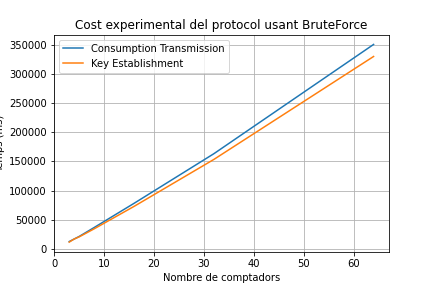
\includegraphics[width=\textwidth]{imgs/cost/brute.png}
	\end{subfigure}
\begin{subfigure}[b]{0.47\textwidth}
	\centering
	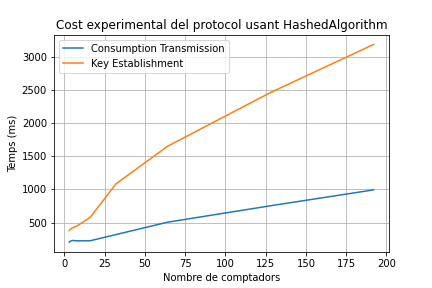
\includegraphics[width=\textwidth]{imgs/cost/hashed.png}
\end{subfigure}
\begin{subfigure}[b]{0.47\textwidth}
	\centering
	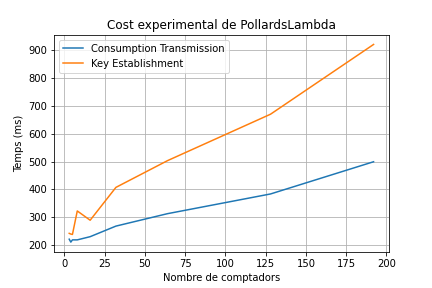
\includegraphics[width=\textwidth]{imgs/cost/pollards.png}
\end{subfigure}
	\caption{Costos experimentals de les fases en funció dels algoritmes}
	\label{fig:algorithms}
\end{figure}
Per tal de verificar que el cost del logaritme discret és exponencial i veure més detalladament el cost de cada algoritme, s'ha analitzat el cost de l'algoritme en funció del nombre de bits del missatge, d'aquesta manera, perdem el coll d'ampolla a la sincronia.
\begin{figure}[H]
	\centering
	\begin{subfigure}[b]{0.48\textwidth}
		\centering
		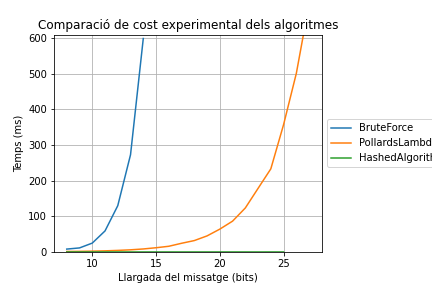
\includegraphics[width=7cm]{imgs/cost/algoritmes-cost.png}
	\end{subfigure}
	\begin{subfigure}[b]{0.48\textwidth}
	\centering
	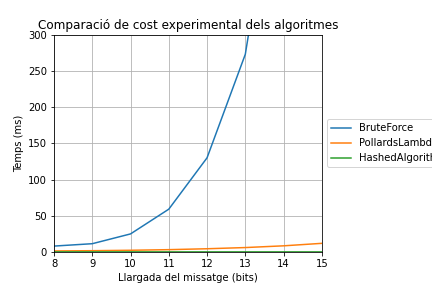
\includegraphics[width=7cm]{imgs/cost/algoritmes-cost2.png}
	\end{subfigure}
	\caption{Comparació dels costos experimentals dels algoritmes en funció del nombre de bits.}
	\label{fig:cost-algo}
\end{figure}
Encara que l'algoritme cachejat tingui un cost teòric $\mathcal{O}(1)$ a l'hora de buscar el logaritme discret, té una càrrega inicial exponencial segons el nombre de bits que es vulgui agafar. Si es busca algun logaritme el resultat el qual s'escapi d'aquests bits, aquest no el podrà trobar.
\begin{figure}[H]
	\centering
	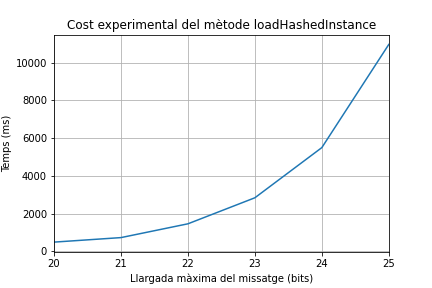
\includegraphics[width=8cm]{imgs/cost/pollardslambda.png}
	\caption{Cost experimental del mètode \texttt{loadHashedInstance}.}
	\label{fig:pollardslambda}
\end{figure}
A més a més, és important l'ús de la memòria principal en aquest tipus d'algoritmes, ja que guardant $2^{20}$ relacions, s'ha necessitat \texttt{1 GB} en memòria.
\section{Comparació de Busom i RECSI}
S'ha volgut comparar en funció del temps els protocols \cite{recsi} i \cite{busom}. A mesura que van augmentar el nombre de comptadors i, per conseqüència, el nombre de bits del missatge agregat, es pot veure a la \textit{Figura \ref{fig:prottime}} que els dos tenen un comportament exponencial. No obstant això, es pot veure com en \cite{recsi}, té una corba menys pronunciada, ja que en la fase de transmissió del consum no es necessita de tanta comunicació com a \cite{busom}. També cal esmentar, que \cite{recsi} és millor quan més lectures són enviades, ja que sí que el seu cost d'establiment de claus és més elevat. Per aquest motiu si el nombre de lectures a enviar de cada comptador, és a dir, el nombre de rondes $R$ de transmissió de lectures, és més petit que els chunks a enviar, és aconsellable usar el protocol \cite{busom}.
\[R \le |Chunks|, \qquad |Chunks| = \frac{\textrm{ordre de la corba}}{\#\textrm{chunk}_2} = \frac{\textrm{ordre de la corba}}{13}\]
\begin{figure}[H]
	\centering
	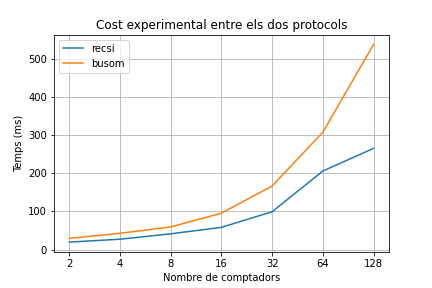
\includegraphics[width=8cm]{imgs/cost/prottime.png}
	\caption{Cost experimental dels protocols \cite{recsi} i \cite{busom}.}
	\label{fig:prottime}
\end{figure}
\begin{table}[H]
	\centering
	\begin{tabular}{l|rr}
		Meters & SSt-BS (ms) & SSt-CT (ms) \\ \hline
		2      &     27.9333 &     19.5500 \\
		4      &     39.7833 &     27.1500 \\
		8      &        56.0 &     41.3667 \\
		16     &     88.6333 &     58.2667 \\
		32     &    156.9167 &     99.3500 \\
		64     &    283.4833 &    206.2667 \\
		128    &    485.8333 &      265.70
	\end{tabular}
	\caption{Mitjana de la subestació realitzant el logaritme discret.}
	\label{ana:tab1}
\end{table}
\end{document}